\section{Results}
\label{sec:results}

\subsection{PCC count and luminosity}

\begin{figure}[H]
  \centering
  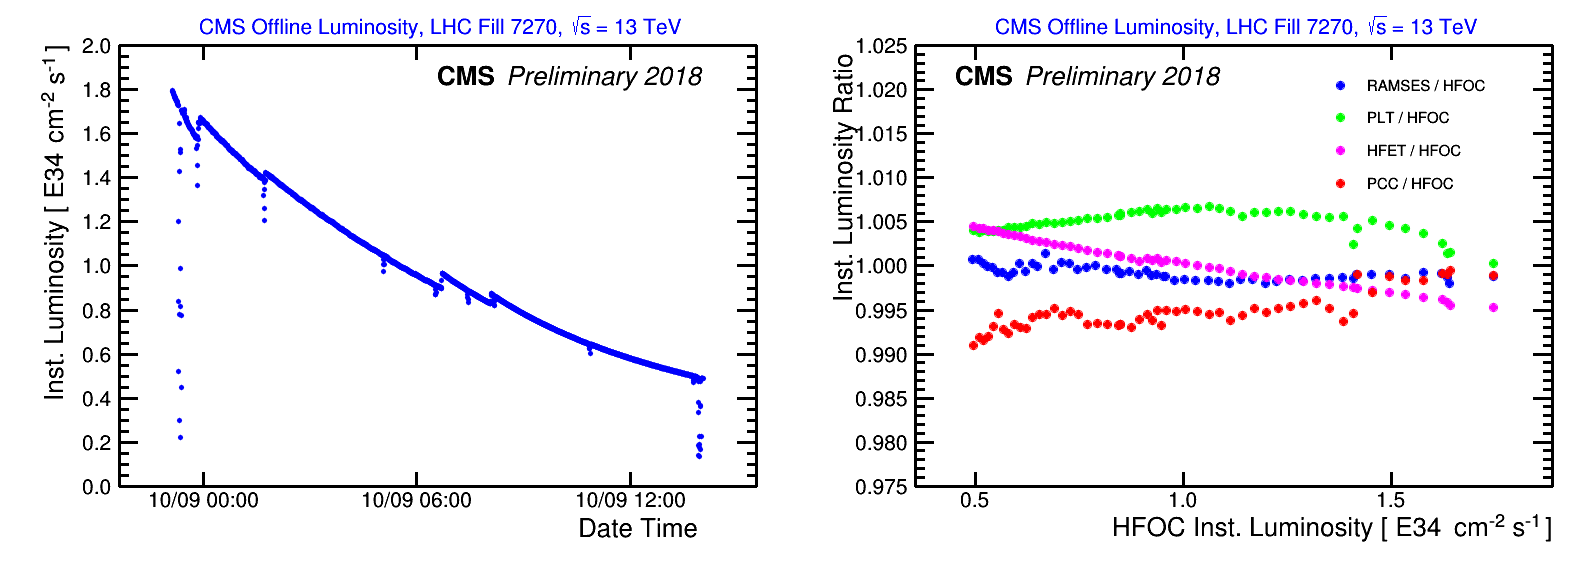
\includegraphics[width=1\columnwidth]{./lhcfill_t.png}
  \caption{Left: Instantaneous luminosity as measured offline by the HFOC luminometer for LHC fill 7270. Right: Ratios of instantaneous luminosity as measured offline by the CMS luminometers as a function of instantaneous luminosity measured by HFOC.}
  \label{fig:CMS}
\end{figure}

PCC cluster counts and calculated integrated luminosity after applying luminosity calibration (visible cross section) for Run2018 A, B and C are shown below.

 \begin{figure}[H]
  \centering
  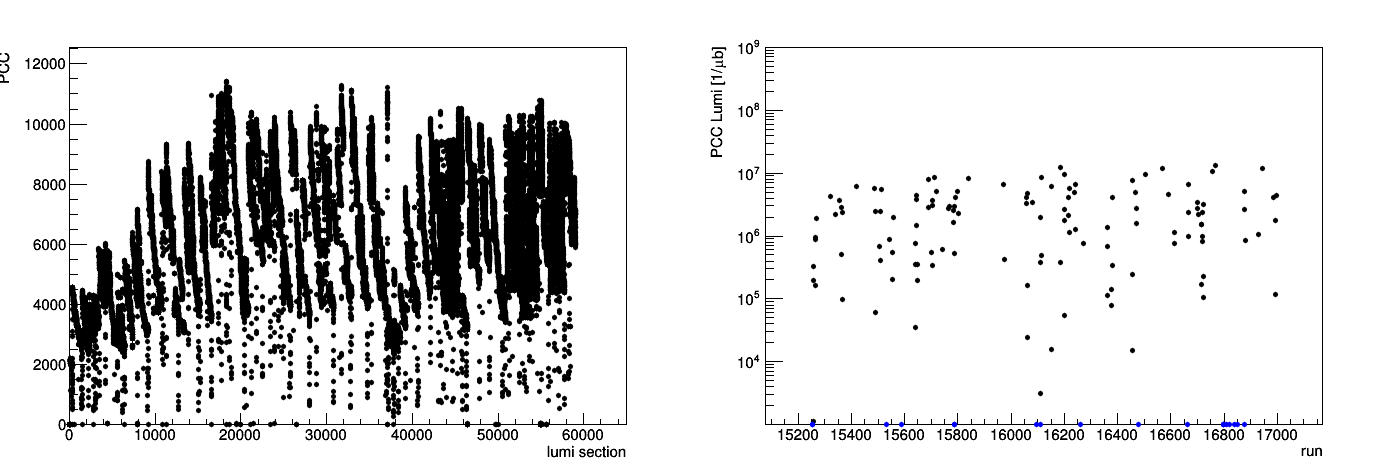
\includegraphics[width=1\columnwidth]{./lumiA_merged.png}
  \caption{Left: PCC count as a function of luminosity section (1 lumi section is 23.36s) for Run2018A. Right: PCC integrated luminosity ($\mu b^{-1}$) as a function of run number for Run2018A.}
  \label{fig:CMS}
\end{figure}


\begin{figure}[H]
  \centering
  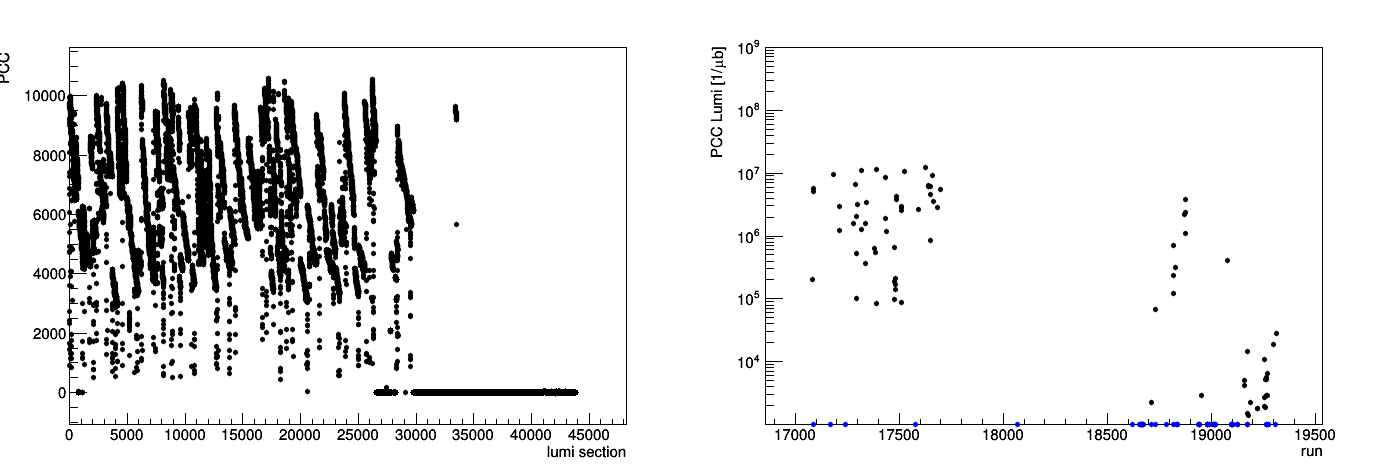
\includegraphics[width=1\columnwidth]{./lumiB_merged.png}
  \caption{Left: PCC count as a function of lumi section for Run2018B. Right: PCC integrated luminosity ($\mu b^{-1}$) as a function of run number for Run2018B}
  \label{fig:CMS}
\end{figure}

\begin{figure}[H]
  \centering
  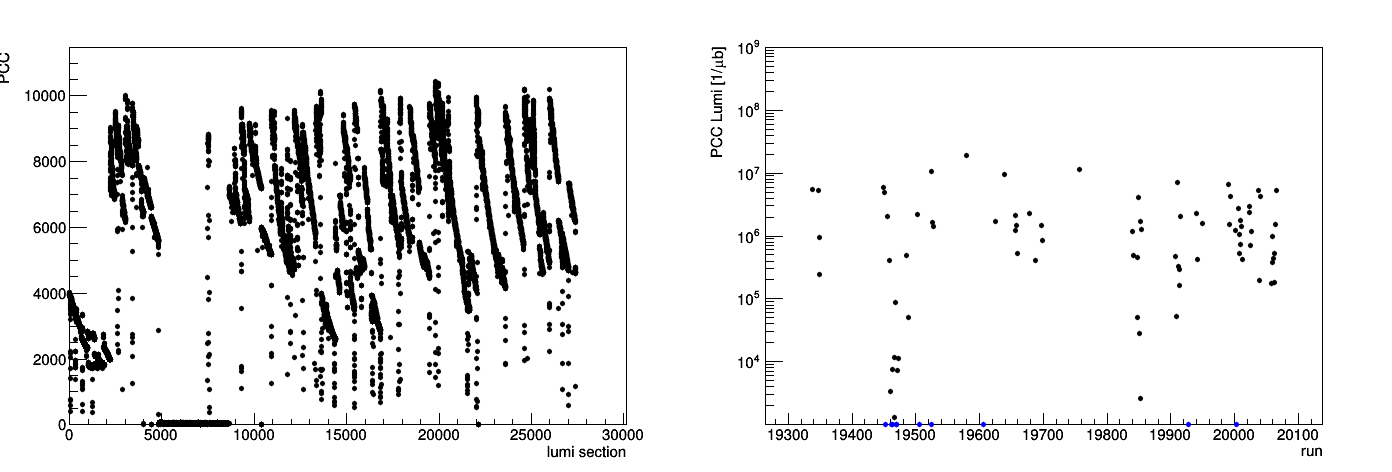
\includegraphics[width=1\columnwidth]{./lumiC_merged.png}
  \caption{Left: PCC count as a function of lumi section for Run2018C. Right: PCC integrated luminosity ($\mu b^{-1}$) as a function of run number for Run2018C.}
  \label{fig:CMS}
\end{figure}


\subsection{Stability of PCC luminosity for Run 2018 CMS data}

The stability of run 2018 CMS integrated luminosity for Phase I pixel detector calculated using PCC method is investigated by employing late Run2018D veto list and including afterglow effects. Luminosity ratios for various subdetectors in pixel detector are computed with respect to total pixel detector luminosity after applying module veto lists for each subdetector. New module selections will be determined and used for 2018 luminosity determination. 
\begin{figure}[H]
  \centering
  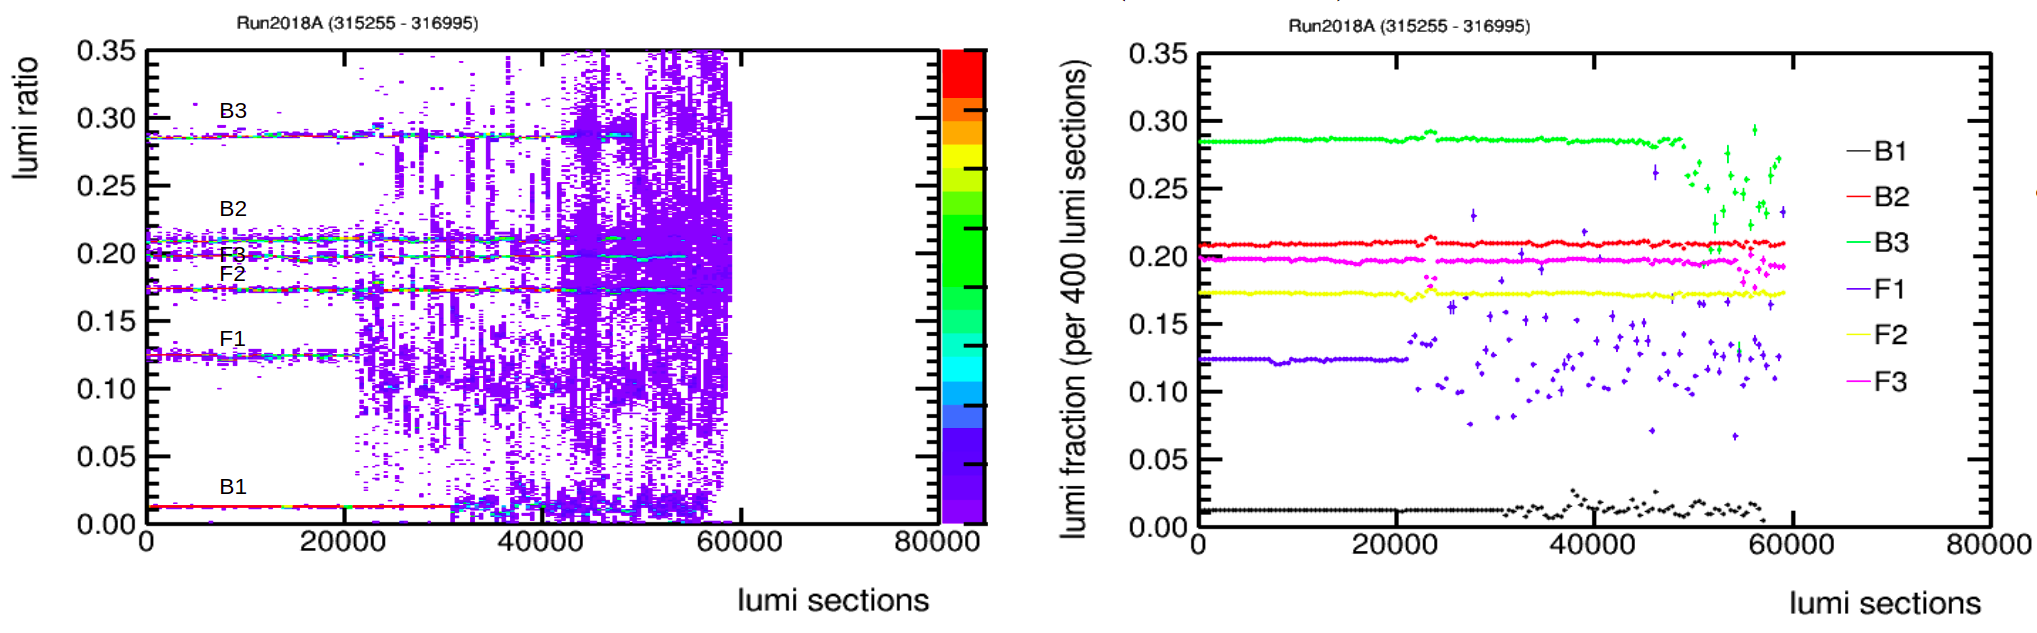
\includegraphics[width=1\columnwidth]{./t25ld-kgsjf.png}
  \caption{Left: Luminosity ratios for various subdetectors L2, L3, L4, D1, D2, D3 of pixel detector as a function of lumi section for Run2018A. Right: X Profile of luminosity ratios vs lumi section graph for various subdetectors L2, L3, L4, D1, D2, D3 of pixel detector showing luminosity fraction as a function of lumi section (1 lumi section is 23.36s) for Run2018A.}
  \label{fig:CMS}
\end{figure}


\begin{figure}[H]
  \centering
  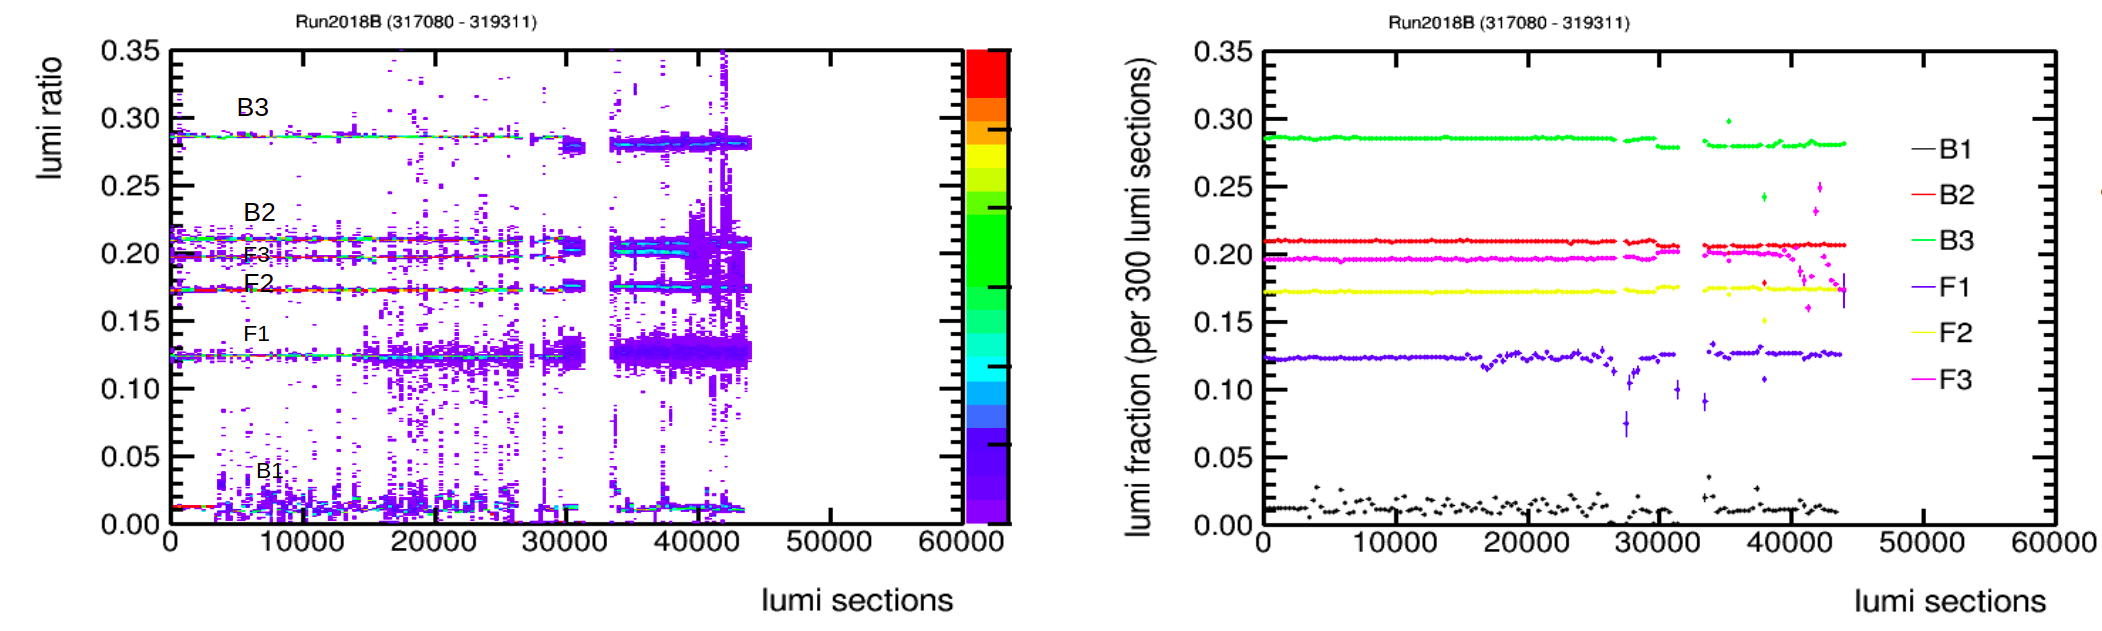
\includegraphics[width=1\columnwidth]{./tjag3-rger6.png}
  \caption{Left: Luminosity ratios for various subdetectors L2, L3, L4, D1, D2, D3 of pixel detector as a function of lumi section for Run2018B. Right: X Profile of luminosity ratios vs lumi section graph for various subdetectors L2, L3, L4, D1, D2, D3 of pixel detector showing luminosity fraction as a function of lumi section for Run2018B. }
  \label{fig:CMS}
\end{figure}



\begin{figure}[H]
  \centering
  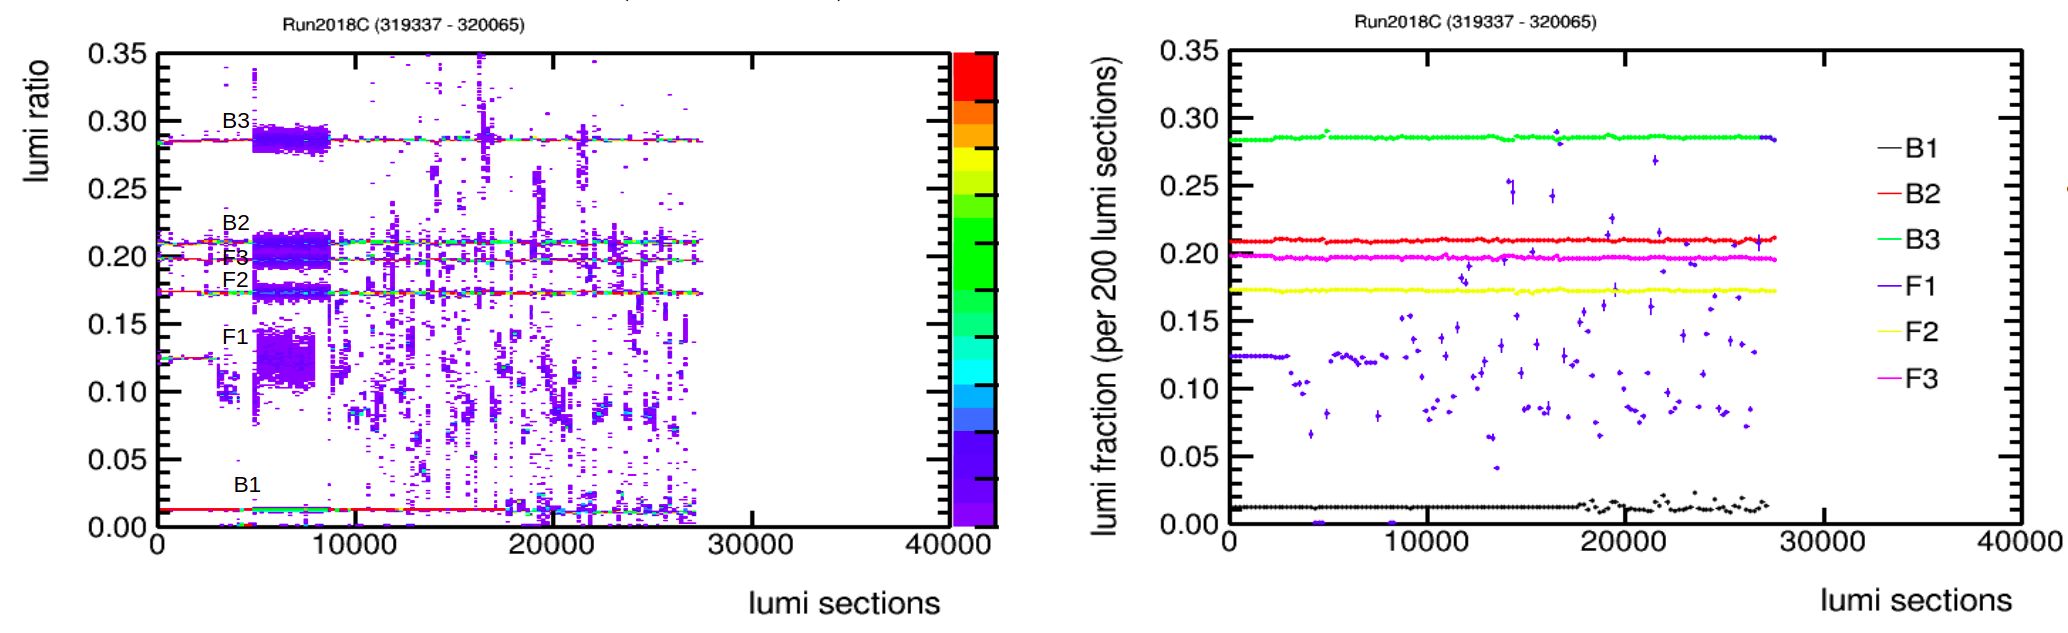
\includegraphics[width=1\columnwidth]{./tfkx3-uyzgt.png}
  \caption{Left: Luminosity ratios for various subdetectors L2, L3, L4, D1, D2, D3 of pixel detector as a function of lumi section for Run2018C. Right: X Profile of luminosity ratios vs lumi section graph for various subdetectors L2, L3, L4, D1, D2, D3 of pixel detector showing luminosity fraction as a function of lumi section for Run2018C \cite{lumidpg}.}
  \label{fig:CMS}
\end{figure}




\clearpage\newpage
